Za potrebe ovog rada izgrađen je sustav za klasifikaciju rukom pisanih slova hrvatske abecede koji se temelji na konvolucijskoj neuronskoj mreži. Sama mreža je izgrađena, učena i evaluirana korištenjem biblioteke \emph{Keras}. \emph{Keras} je biblioteka pisana u programskom jeziku \emph{Python} koja nudi vrlo jednostavno programsko sučelje za izgradnju neuronskih mreža i širok spektar algoritama za učenje iste.

\section{Skup podataka}

Za potrebe učenja klasifikatora, to jest konvolucijske neuronske mreže, prikupljen je skup podataka od \num{16000} slika slova hrvatske abecede i znakova, i to \num{7750} velikih i \num{7750} malih slova te \num{500} primjera znaka "-" koji bi služio kao oznaka poništavanja odgovora ukoliko bi se navedeni sustav koristio prilikom ispravljanja ispita s abc-pitalicama.

Skup podataka je podijeljen na 63 razreda, gdje svaki razred određuje jedan znak. Pa su tako iz hrvatske abecede izbačena slova koja se mogu dobiti kombinacijom više znakova (lj, nj i dž) te su, uz spomenuti znak "-", dodana i slova engleske abecede (x, y, w i q).

Prikupljanje skupa podataka se obavljalo preko predefiniranih obrazaca gdje je svaka osoba trebala upisati po deset varijanti malog slova, te deset varijanti velikog slova što ukupno daje 640 znakova po osobi. Obrasci su skenirani u nijansama sivih boja te su se zatim sva slova automatizirano izrezivala i svrstavala u određeni razred.

Na tako izlučenom skupu slika slova obavljalo se pretprocesiranje i to u sljedećim koracima:

 \begin{enumerate}
   \item binarizacija slike slova koristeći \emph{Otsu-ovu} metodu, 
   \item segmentacija slova od ruba do ruba tako da se izbaci što veći dio pozadine te
   \item skaliranje tako izvučenog slova na dimenzije $30 \times 30$ slikovnih elemenata uz očuvanje omjera širine i visine slova.
 \end{enumerate}

Primjer obrađenih slova iz skupa podataka se može vidjeti na slici \ref{fig:dataset_example}.

\begin{figure}[htb]
    \centering
    
\includegraphics[width=11.5cm]{images/dataset_example.pdf}
    \caption{Primjer obrađenih slova iz skupa podataka.}
    \label{fig:dataset_example}
\end{figure}

\section{Arhitektura mreže}

Kako je navedeno u prijašnjem potpoglavlju, krajnja veličina slike slova je $30 \times 30$ slikovnih elemenata, stoga i mreža korištena u ovom radu na svom prvom sloju ima $900$ ulaznih točaka. Na svom izlazu mreža ima $32$ neurona. Broj izlaza je manji nego broj samih razreda slova (velikih i malih) zbog toga što navedeni sustav na izlazu ne razlikuje velika i mala slova, na primjer veliko slovo A i malo slovo a klasificira u isti razred. Razlog takvog ''pojednostavljenja'' klasifikacije leži u tome što mreža na svom ulazu dobiva čistu sliku slova, bez poznavanja konteksta u kojem se to slovo pojavilo pa bi samoj mreži bilo iznimno teško, pa čak i nemoguće, razlučiti radi li se na primjer o velikom slovu O ili malom slovu o.

Prilikom učenja klasifikatora isprobano je nekoliko različitih arhitektura konvolucijskih neuronskih mreža, no najbolji rezultati su ostvareni uz arhitekturu kod koje je poredak pojedinih slojeva bio sljedeći:

\begin{enumerate}
    \item ulazni konvolucijski sloj s $32$ filtra dimenzije $3 \times 3$ i korakom pomaka jednakim $1$, uz korištenje \emph{ReLU} aktivacijske funkcije,
    \item sloj sažimanja maksimalnom vrijednosti uz veličinu filtra $2 \times 2$,
    \item konvolucijski sloj s $64$ filtra dimenzije $3 \times 3$ i korakom pomaka jednakim $1$, uz korištenje \emph{ReLU} aktivacijske funkcije,
    \item sloj sažimanja maksimalnom vrijednosti uz veličinu filtra $2 \times 2$,
    \item potpuno povezani sloj s $128$ neurona gdje svaki neuron koristi \emph{ReLU} aktivacijsku funkciju na svom izlazu,
    \item još jedan potpuno povezani sloj identičan prijašnjem te
    \item izlazni sloj s $32$ neurona koji na svom izlazu koriste \emph{softmax} aktivacijsku funkciju.
\end{enumerate}

\section{Učenje mreže}

Učenje konvolucijske neuronske mreže obavljalo se na grafičkoj kartici \emph{NVIDIA Tesla K80} što je uvelike ubrzalo sam proces učenja. Usporedbe radi, prilikom učenja korištenjem samo procesora jedna epoha učenja je trajala u prosjeku 45 sekundi, dok se uz uporabu navedene grafičke kartice jedna epoha spustila na svega dvije sekunde u prosjeku.

Za potrebe učenja ulazni skup podataka se podijelio na tri podskupa: skup za učenje, skup za provjeru te skup za ispitivanje. Skup za učenje se sastojao od \num{12000} uzoraka, skup za provjeru od \num{3000} uzoraka te skup za ispitivanje od \num{1000} uzoraka. Na skupu za učenje, kako mu i ime govori, se učila konvolucijska neuronska mreža, skup za provjeru se koristio za odabir modela, to jest mreže s optimalnim parametrima, dok se na skupu za testiranje provjeravala točnost samog odabranoga modela.

Zbog relativno malog broja uzoraka u skupu za učenje korištena je augmentacija podataka tokom učenja mreže. Prije dovođenja uzorka na ulaze mreže tokom učenja, svaki se uzorak s određenom vjerojatnošću modificirao i to na način da bi se rotirao za nekoliko stupnjeva u lijevo ili desno (gornja granica je postavljena na osam stupnjeva u oba smjera) i/ili bi se slovo na slici pomicalo gore/dolje i/ili lijevo/desno za maksimalno $10\%$ svoje visine/širine.

Tokom učenja kao funkcija gubitka korištena je kategorička unakrsna entropija, a za samo učenje korištena je metoda \emph{ADADELTA} opisana u radu \citep{adadelta}. Prednost navedene metode učenja je to što ne zahtjeva ručni odabir stope učenja, već ju dinamički određuje prilikom samog učenja.

U prvih nekoliko pokušaja učenja mreže nisu korištene nikakve regularizacijske tehnike što je dovelo prenaučenosti same mreže u svega nekoliko epoha. Vrijednost funkcije gubitka takvog modela kroz epohe vidljiva je na slici \ref{fig:overfit} gdje se lako uočava brzi porast greške na skupu za provjeru. 

\begin{figure}[htb]
    \centering
    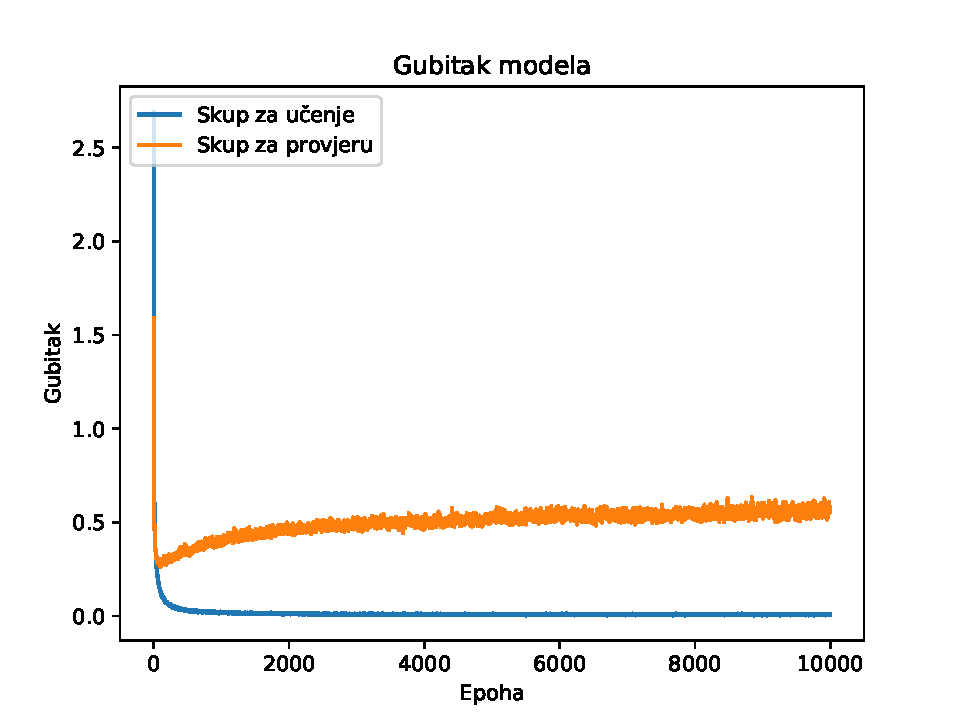
\includegraphics[width=12cm]{images/overfit.pdf}
    \caption{Gubitak prenaučenog modela}
    \label{fig:overfit}
\end{figure}

Kako bi se doskočilo problemu prenaučenosti same mreže, potrebno je uvesti neke regularizacijske tehnike. Najčešće korištena tehnika kod konvolucijskih neuronskih mreža je \emph{dropout} opisana u radu \citep{dropout}. Sam pojam \emph{dropout} se odnosi na ''ispuštanje'' skrivenih ili vanjskih čvorova, u ovom slučaju neurona ili samih filtra konvolucijskog sloja ili sloja sažimanja. ''Ispuštanje'' u kontekstu konvolucijskih neuronskih mreža predstavlja odspajanje pojedinog filtra ili neurona sa svih svojih ulaza i izlaza. Na taj način čvor postaje manje osjetljiv na promjene težina i time se dobiva robusniji model. Sam odabir čvora koji će se ispustiti tokom učenja je slučajan, te sama vjerojatnost ''ispuštanja'' čvora predstavlja hiperparametar modela prilikom faze učenja.

Za arhitekturu konvolucijske neuronske mreže navedenu u prijašnjem potpoglavlju, \emph{dropout} je dodan između zadnjeg sloja sažimanja i prvog potpuno povezanoga sloja i to s vjerojatnošću ispuštanja $0.25$, te između prvog i drugog potpuno povezanoga sloja s vjerojatnošću ispuštanja $0.5$. Tako učena mreža ostvarila je najbolje rezultate. Prikaz vrijednosti funkcije gubitka takve mreže kroz epohe za pojedine skupove vidljiv je na slici \ref{fig:model_loss}, dok se točnost klasifikacije kroz epohe može promatrati na slici \ref{fig:model_acc}.

\begin{figure}[!htbp]
    \centering
    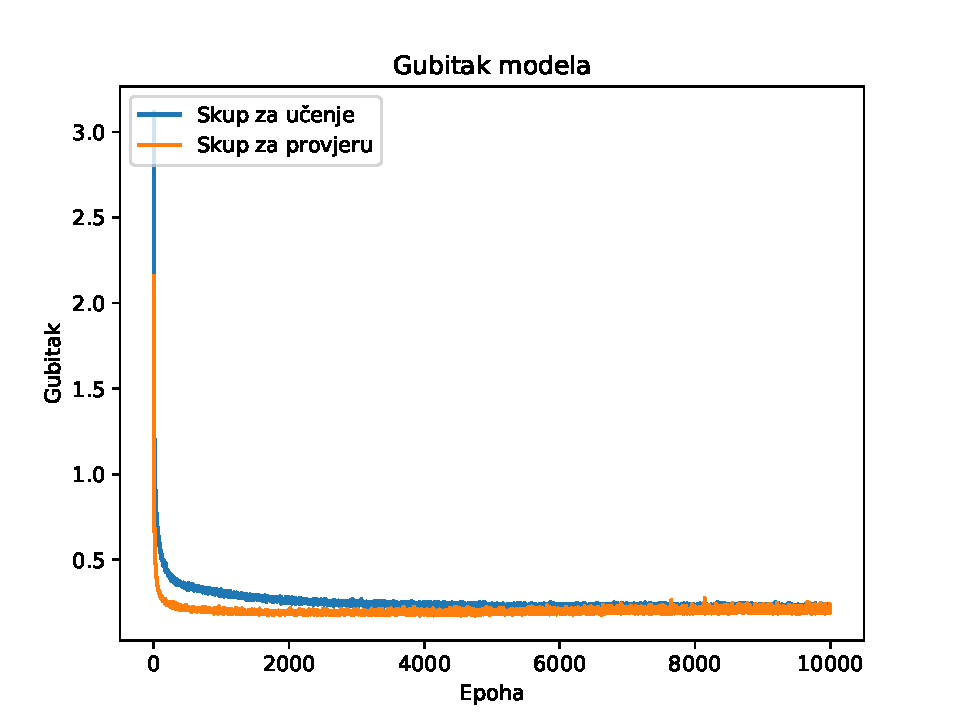
\includegraphics[width=12cm]{images/model_loss.pdf}
    \caption{Gubitak modela}
    \label{fig:model_loss}
\end{figure}

\begin{figure}[!htbp]
    \centering
    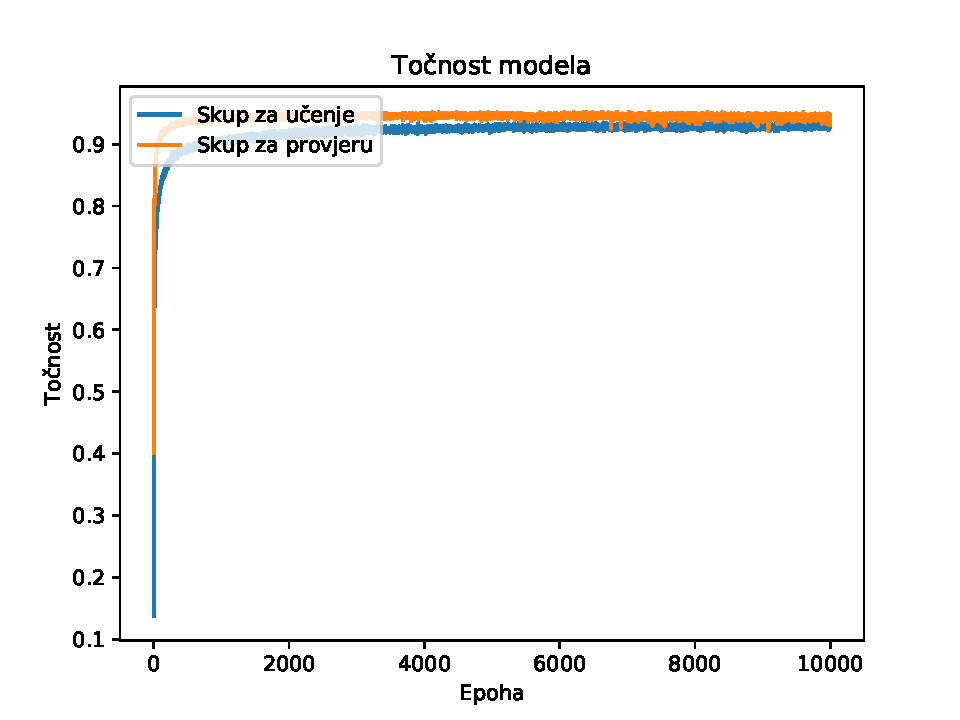
\includegraphics[width=12cm]{images/model_acc.pdf}
    \caption{Točnost klasifikacije modela}
    \label{fig:model_acc}
\end{figure}

\section{Rezultati}

Najbolji rezultati su ostvareni na konvolucijskoj neuronskoj mreži opisanoj u jednom od prijašnjih poglavlja uz već navedene postupke učenja i tehnika regularizacije. Točnost klasifikacije modela na skupu za testiranje iznosila je $94\%$, što znači da je svega $60$ od $1000$ primjera iz skupa za ispitivanje krivo klasificirano.

Primjer krivo klasificiranih primjera iz skupa za ispitivanje vidljiv je na slici \ref{fig:wrong_class}. Može se uočiti kako najviše problema uzrokuju kombinacije malog slova l i velikog slova I, malog slova h i malog slova n, slova u i slova v. No, među danim primjerima se mogu uočiti i krivo napisana slova, poput obrnutog slova N, slova E bez donje crtice i slični. Za velik broj slučajeva s navedene slike ni sam čovjek ne bi mogao točno razlučiti o kojem je slovu riječ bez poznavanja šireg konteksta u kojem se to slovo pojavilo.

\begin{figure}[htb]
    \centering
    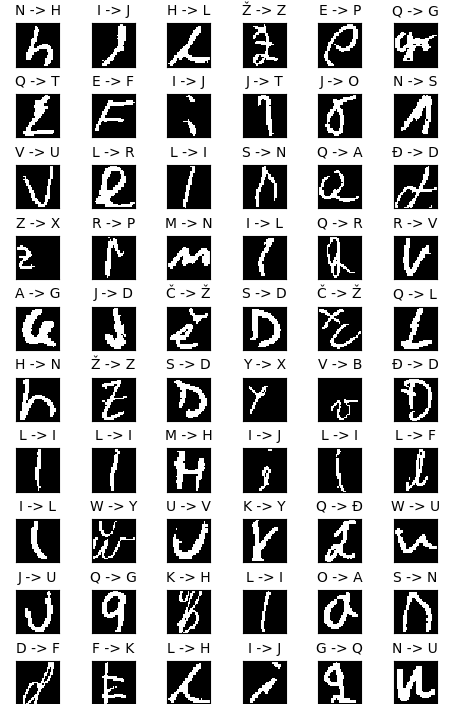
\includegraphics[width=10cm]{images/wrong.png}
    \caption{Krivo klasificirani primjeri iz skupa za ispitivanje. Lijeva strana izraza predstavlja stvarnu oznaku, a desna izlaz klasifikatora.}
    \label{fig:wrong_class}
\end{figure}

Tablicom \ref{confusion_matrix_cro} prikazana je matrica zabune na ispitnom skupu gdje pojedini element iz tablice predstavlja broj koliko je puta slovo iz retka prepoznato kao slovo iz stupca.
 
\begin{table}[]
\setlength{\tabcolsep}{2pt}
\centering
\caption{Matrica zabune za hrvatsku abecedu. Element tablice predstavlja broj koliko je puta slovo iz retka prepoznato kao slovo iz stupca.}
\label{confusion_matrix_cro}
\scalebox{0.75} {
\begin{tabular}{|c|c|c|c|c|c|c|c|c|c|c|c|c|c|c|c|c|c|c|c|c|c|c|c|c|c|c|c|c|c|c|c|c|}
\cline{1-33}
/ & A & B & C & Č & Ć & D & Đ & E & F & G & H & I & J & K & L & M & N & O & P & R & S & Š & T & U & V & Z & Ž & X & Y & W & Q & - \\ \hline \rowcolor{gray1}
A & \textbf{34} & 0 & 0 & 0 & 0 & 0 & 0 & 0 & 0 & 1 & 0 & 0 & 0 & 0 & 0 & 0 & 0 & 0 & 0 & 0 & 0 & 0 & 0 & 0 & 0 & 0 & 0 & 0 & 0 & 0 & 0 & 0 \\ \hline \rowcolor{gray2} 
B & 0 & \textbf{31} & 0 & 0 & 0 & 0 & 0 & 0 & 0 & 0 & 0 & 0 & 0 & 0 & 0 & 0 & 0 & 0 & 0 & 0 & 0 & 0 & 0 & 0 & 0 & 0 & 0 & 0 & 0 & 0 & 0 & 0 \\ \hline \rowcolor{gray1}
C & 0 & 0 & \textbf{29} & 0 & 0 & 0 & 0 & 0 & 0 & 0 & 0 & 0 & 0 & 0 & 0 & 0 & 0 & 0 & 0 & 0 & 0 & 0 & 0 & 0 & 0 & 0 & 0 & 0 & 0 & 0 & 0 & 0 \\ \hline \rowcolor{gray2} 
Č & 0 & 0 & 0 & \textbf{30} & 0 & 0 & 0 & 0 & 0 & 0 & 0 & 0 & 0 & 0 & 0 & 0 & 0 & 0 & 0 & 0 & 0 & 0 & 0 & 0 & 0 & 0 & 2 & 0 & 0 & 0 & 0 & 0 \\ \hline \rowcolor{gray1}
Ć & 0 & 0 & 0 & 0 & \textbf{28} & 0 & 0 & 0 & 0 & 0 & 0 & 0 & 0 & 0 & 0 & 0 & 0 & 0 & 0 & 0 & 0 & 0 & 0 & 0 & 0 & 0 & 0 & 0 & 0 & 0 & 0 & 0 \\ \hline \rowcolor{gray2} 
D & 0 & 0 & 0 & 0 & 0 & \textbf{31} & 0 & 0 & 1 & 0 & 0 & 0 & 0 & 0 & 0 & 0 & 0 & 0 & 0 & 0 & 0 & 0 & 0 & 0 & 0 & 0 & 0 & 0 & 0 & 0 & 0 & 0 \\ \hline \rowcolor{gray1}
Đ & 0 & 0 & 0 & 0 & 0 & 2 & \textbf{27} & 0 & 0 & 0 & 0 & 0 & 0 & 0 & 0 & 0 & 0 & 0 & 0 & 0 & 0 & 0 & 0 & 0 & 0 & 0 & 0 & 0 & 0 & 0 & 0 & 0 \\ \hline \rowcolor{gray2} 
E & 0 & 0 & 0 & 0 & 0 & 0 & 0 & \textbf{31} & 1 & 0 & 0 & 0 & 0 & 0 & 0 & 0 & 0 & 0 & 1 & 0 & 0 & 0 & 0 & 0 & 0 & 0 & 0 & 0 & 0 & 0 & 0 & 0 \\ \hline \rowcolor{gray1}
F & 0 & 0 & 0 & 0 & 0 & 0 & 0 & 0 & \textbf{34} & 0 & 0 & 0 & 0 & 1 & 0 & 0 & 0 & 0 & 0 & 0 & 0 & 0 & 0 & 0 & 0 & 0 & 0 & 0 & 0 & 0 & 0 & 0 \\ \hline \rowcolor{gray2} 
G & 0 & 0 & 0 & 0 & 0 & 0 & 0 & 0 & 0 & \textbf{30} & 0 & 0 & 0 & 0 & 0 & 0 & 0 & 0 & 0 & 0 & 0 & 0 & 0 & 0 & 0 & 0 & 0 & 0 & 0 & 0 & 1 & 0 \\ \hline \rowcolor{gray1}
H & 0 & 0 & 0 & 0 & 0 & 0 & 0 & 0 & 0 & 0 & \textbf{22} & 0 & 0 & 0 & 1 & 0 & 1 & 0 & 0 & 0 & 0 & 0 & 0 & 0 & 0 & 0 & 0 & 0 & 0 & 0 & 0 & 0 \\ \hline \rowcolor{gray2} 
I & 0 & 0 & 0 & 0 & 0 & 0 & 0 & 0 & 0 & 0 & 0 & \textbf{25} & 4 & 0 & 2 & 0 & 0 & 0 & 0 & 0 & 0 & 0 & 0 & 0 & 0 & 0 & 0 & 0 & 0 & 0 & 0 & 0 \\ \hline \rowcolor{gray1}
J & 0 & 0 & 0 & 0 & 0 & 1 & 0 & 0 & 0 & 0 & 0 & 0 & \textbf{21} & 0 & 0 & 0 & 0 & 1 & 0 & 0 & 0 & 0 & 1 & 1 & 0 & 0 & 0 & 0 & 0 & 0 & 0 & 0 \\ \hline \rowcolor{gray2} 
K & 0 & 0 & 0 & 0 & 0 & 0 & 0 & 0 & 0 & 0 & 1 & 0 & 0 & \textbf{32} & 0 & 0 & 0 & 0 & 0 & 0 & 0 & 0 & 0 & 0 & 0 & 0 & 0 & 0 & 1 & 0 & 0 & 0 \\ \hline \rowcolor{gray1}
L & 0 & 0 & 0 & 0 & 0 & 0 & 0 & 0 & 1 & 0 & 1 & 5 & 0 & 0 & \textbf{31} & 0 & 0 & 0 & 0 & 1 & 0 & 0 & 0 & 0 & 0 & 0 & 0 & 0 & 0 & 0 & 0 & 0 \\ \hline \rowcolor{gray2} 
M & 0 & 0 & 0 & 0 & 0 & 0 & 0 & 0 & 0 & 0 & 1 & 0 & 0 & 0 & 0 & \textbf{32} & 1 & 0 & 0 & 0 & 0 & 0 & 0 & 0 & 0 & 0 & 0 & 0 & 0 & 0 & 0 & 0 \\ \hline \rowcolor{gray1}
N & 0 & 0 & 0 & 0 & 0 & 0 & 0 & 0 & 0 & 0 & 1 & 0 & 0 & 0 & 0 & 0 & \textbf{27} & 0 & 0 & 0 & 1 & 0 & 0 & 1 & 0 & 0 & 0 & 0 & 0 & 0 & 0 & 0 \\ \hline \rowcolor{gray2} 
O & 1 & 0 & 0 & 0 & 0 & 0 & 0 & 0 & 0 & 0 & 0 & 0 & 0 & 0 & 0 & 0 & 0 & \textbf{23} & 0 & 0 & 0 & 0 & 0 & 0 & 0 & 0 & 0 & 0 & 0 & 0 & 0 & 0 \\ \hline \rowcolor{gray1}
P & 0 & 0 & 0 & 0 & 0 & 0 & 0 & 0 & 0 & 0 & 0 & 0 & 0 & 0 & 0 & 0 & 0 & 0 & \textbf{26} & 0 & 0 & 0 & 0 & 0 & 0 & 0 & 0 & 0 & 0 & 0 & 0 & 0 \\ \hline \rowcolor{gray2} 
R & 0 & 0 & 0 & 0 & 0 & 0 & 0 & 0 & 0 & 0 & 0 & 0 & 0 & 0 & 0 & 0 & 0 & 0 & 1 & \textbf{35} & 0 & 0 & 0 & 0 & 1 & 0 & 0 & 0 & 0 & 0 & 0 & 0 \\ \hline \rowcolor{gray1}
S & 0 & 0 & 0 & 0 & 0 & 2 & 0 & 0 & 0 & 0 & 0 & 0 & 0 & 0 & 0 & 0 & 2 & 0 & 0 & 0 & \textbf{28} & 0 & 0 & 0 & 0 & 0 & 0 & 0 & 0 & 0 & 0 & 0 \\ \hline \rowcolor{gray2} 
Š & 0 & 0 & 0 & 0 & 0 & 0 & 0 & 0 & 0 & 0 & 0 & 0 & 0 & 0 & 0 & 0 & 0 & 0 & 0 & 0 & 0 & \textbf{45} & 0 & 0 & 0 & 0 & 0 & 0 & 0 & 0 & 0 & 0 \\ \hline \rowcolor{gray1}
T & 0 & 0 & 0 & 0 & 0 & 0 & 0 & 0 & 0 & 0 & 0 & 0 & 0 & 0 & 0 & 0 & 0 & 0 & 0 & 0 & 0 & 0 & \textbf{47} & 0 & 0 & 0 & 0 & 0 & 0 & 0 & 0 & 0 \\ \hline \rowcolor{gray2} 
U & 0 & 0 & 0 & 0 & 0 & 0 & 0 & 0 & 0 & 0 & 0 & 0 & 0 & 0 & 0 & 0 & 0 & 0 & 0 & 0 & 0 & 0 & 0 & \textbf{26} & 1 & 0 & 0 & 0 & 0 & 0 & 0 & 0 \\ \hline \rowcolor{gray1}
V & 0 & 1 & 0 & 0 & 0 & 0 & 0 & 0 & 0 & 0 & 0 & 0 & 0 & 0 & 0 & 0 & 0 & 0 & 0 & 0 & 0 & 0 & 0 & 1 & \textbf{30} & 0 & 0 & 0 & 0 & 0 & 0 & 0 \\ \hline \rowcolor{gray2} 
Z & 0 & 0 & 0 & 0 & 0 & 0 & 0 & 0 & 0 & 0 & 0 & 0 & 0 & 0 & 0 & 0 & 0 & 0 & 0 & 0 & 0 & 0 & 0 & 0 & 0 & \textbf{26} & 0 & 1 & 0 & 0 & 0 & 0 \\ \hline \rowcolor{gray1}
Ž & 0 & 0 & 0 & 0 & 0 & 0 & 0 & 0 & 0 & 0 & 0 & 0 & 0 & 0 & 0 & 0 & 0 & 0 & 0 & 0 & 0 & 0 & 0 & 0 & 0 & 2 & \textbf{26} & 0 & 0 & 0 & 0 & 0 \\ \hline \rowcolor{gray2} 
X & 0 & 0 & 0 & 0 & 0 & 0 & 0 & 0 & 0 & 0 & 0 & 0 & 0 & 0 & 0 & 0 & 0 & 0 & 0 & 0 & 0 & 0 & 0 & 0 & 0 & 0 & 0 & \textbf{29} & 0 & 0 & 0 & 0 \\ \hline \rowcolor{gray1}
Y & 0 & 0 & 0 & 0 & 0 & 0 & 0 & 0 & 0 & 0 & 0 & 0 & 0 & 0 & 0 & 0 & 0 & 0 & 0 & 0 & 0 & 0 & 0 & 0 & 0 & 0 & 0 & 1 & \textbf{23} & 0 & 0 & 0 \\ \hline \rowcolor{gray2} 
W & 0 & 0 & 0 & 0 & 0 & 0 & 0 & 0 & 0 & 0 & 0 & 0 & 0 & 0 & 0 & 0 & 0 & 0 & 0 & 0 & 0 & 0 & 0 & 1 & 0 & 0 & 0 & 0 & 1 & \textbf{23} & 0 & 0 \\ \hline \rowcolor{gray1}
Q & 1 & 0 & 0 & 0 & 0 & 0 & 1 & 0 & 0 & 2 & 0 & 0 & 0 & 0 & 1 & 0 & 0 & 0 & 0 & 1 & 0 & 0 & 1 & 0 & 0 & 0 & 0 & 0 & 0 & 0 & \textbf{23} & 0 \\ \hline \rowcolor{gray2} 
- & 0 & 0 & 0 & 0 & 0 & 0 & 0 & 0 & 0 & 0 & 0 & 0 & 0 & 0 & 0 & 0 & 0 & 0 & 0 & 0 & 0 & 0 & 0 & 0 & 0 & 0 & 0 & 0 & 0 & 0 & 0 & \textbf{35} \\ \hline
\end{tabular}
}
\end{table}